\documentclass[tikz,border=8pt]{standalone}

\usepackage[T1]{fontenc}
\usepackage{lmodern}
\usetikzlibrary{arrows.meta,positioning}

\begin{document}
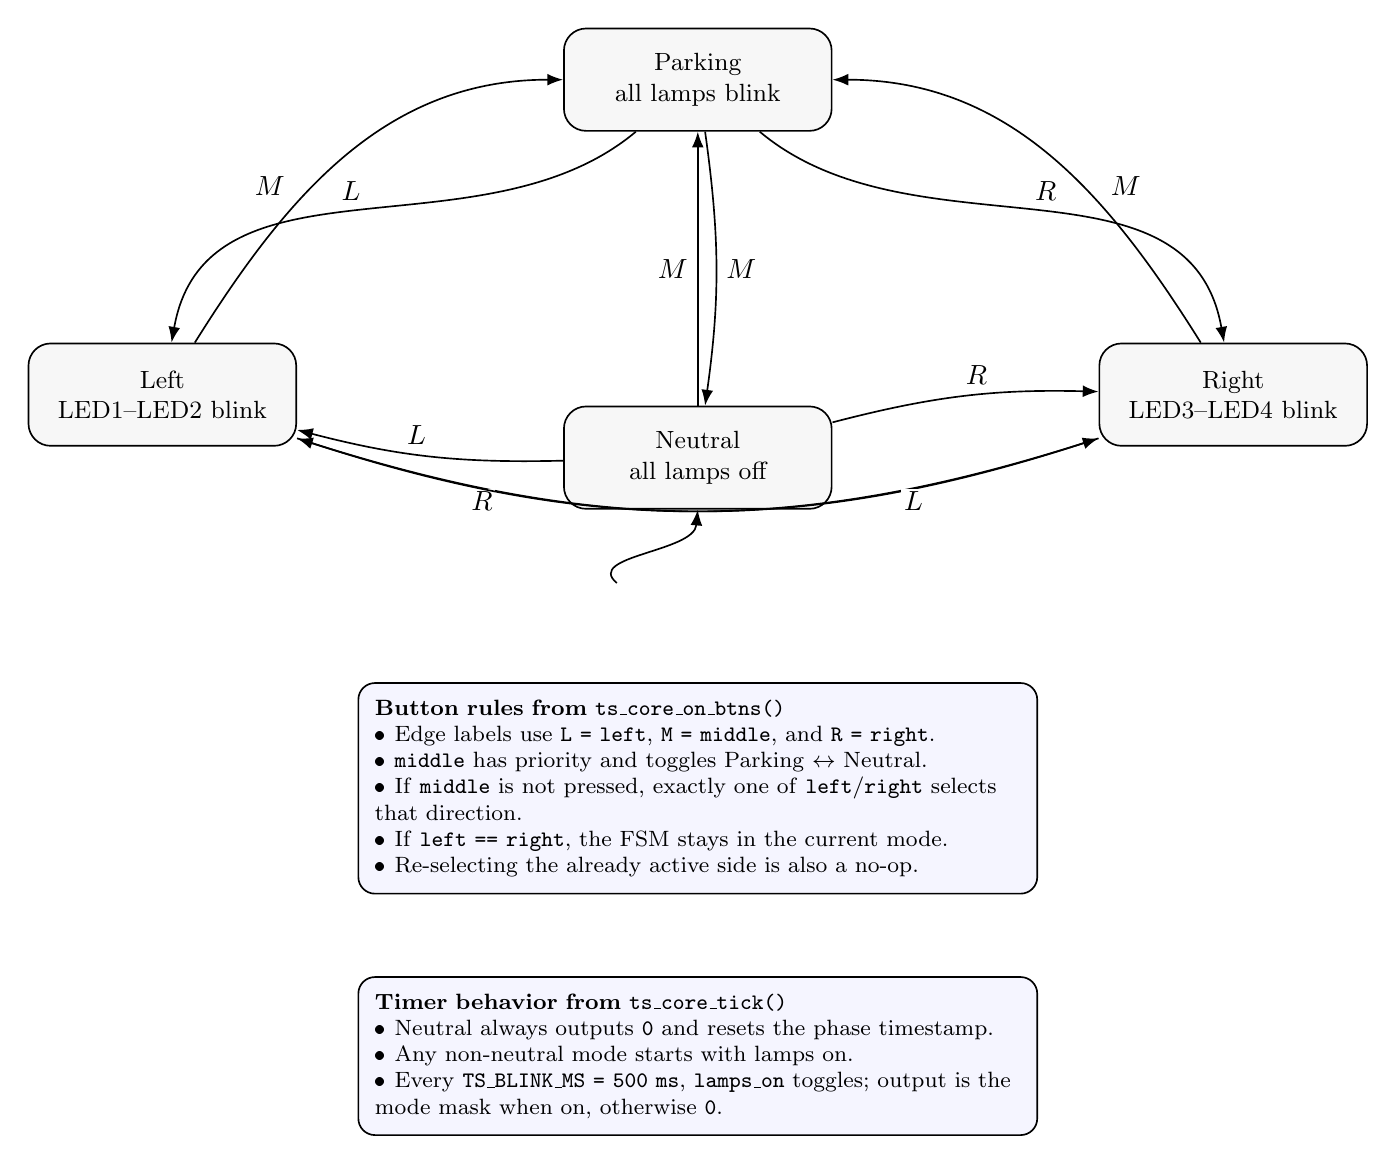
\begin{tikzpicture}[
    >=Latex,
    node distance=34mm,
    semithick,
    state/.style={
        draw,
        rounded corners=8pt,
        minimum width=34mm,
        minimum height=13mm,
        align=center,
        font=\small,
        fill=gray!6
    },
    note/.style={
        draw,
        rounded corners=6pt,
        align=left,
        font=\footnotesize,
        fill=blue!4,
        text width=82mm,
        inner sep=6pt
    }
]

\node[state] (neutral) at (0,-0.8) {Neutral\\all lamps off};
\node[state] (parking) at (0,4.0) {Parking\\all lamps blink};
\node[state] (left) at (-6.8,0) {Left\\LED1--LED2 blink};
\node[state] (right) at (6.8,0) {Right\\LED3--LED4 blink};
\node[draw=none] (start) at (-0.9,-2.5) {};

\path[->]
    (start) edge[out=140, in=-95] (neutral.south)
    (neutral) edge node[left, pos=0.5] {$M$} (parking)
    (neutral) edge[bend left=8] node[above, pos=0.55] {$L$} (left)
    (neutral) edge[bend left=8] node[above, pos=0.55] {$R$} (right)
    (parking) edge[bend left=8] node[right, pos=0.5] {$M$} (neutral)
    (parking) edge[out=220, in=80] node[above left, pos=0.48] {$L$} (left)
    (parking) edge[out=-40, in=100] node[above right, pos=0.48] {$R$} (right)
    (left) edge[out=-18, in=198] node[below, pos=0.22, fill=white, inner sep=1pt] {$R$} (right)
    (left) edge[out=58, in=180] node[above left, pos=0.34] {$M$} (parking)
    (right) edge[out=-162, in=-18] node[below, pos=0.22, fill=white, inner sep=1pt] {$L$} (left)
    (right) edge[out=122, in=0] node[above right, pos=0.34] {$M$} (parking);

\node[note] (rules) at (0,-5.0) {
\textbf{Button rules from \texttt{ts\_core\_on\_btns()}}\\
\textbullet\ Edge labels use \texttt{L = left}, \texttt{M = middle}, and \texttt{R = right}.\\
\textbullet\ \texttt{middle} has priority and toggles Parking $\leftrightarrow$ Neutral.\\
\textbullet\ If \texttt{middle} is not pressed, exactly one of \texttt{left}/\texttt{right} selects that direction.\\
\textbullet\ If \texttt{left == right}, the FSM stays in the current mode.\\
\textbullet\ Re-selecting the already active side is also a no-op.
};

\node[note] (tick) at (0,-8.4) {
\textbf{Timer behavior from \texttt{ts\_core\_tick()}}\\
\textbullet\ Neutral always outputs \texttt{0} and resets the phase timestamp.\\
\textbullet\ Any non-neutral mode starts with lamps on.\\
\textbullet\ Every \texttt{TS\_BLINK\_MS = 500 ms}, \texttt{lamps\_on} toggles; output is the mode mask when on, otherwise \texttt{0}.
};

\end{tikzpicture}
\end{document}
